\documentclass[../report.tex]{subfiles}
\begin{document}

\section{Experiment: Follow Line on the Map} \label{app:line_follower}

\subsection*{Purpose of the Experiment}
To solve the puzzle it is essential for the robot to stay on the lines on the Sokoban map. Therefore, a routine which uses the two color sensors to follow a line is created and tested.
\begin{figure}[H]
    \centering
    \begin{subfigure}{0.5\textwidth}
        \centering
        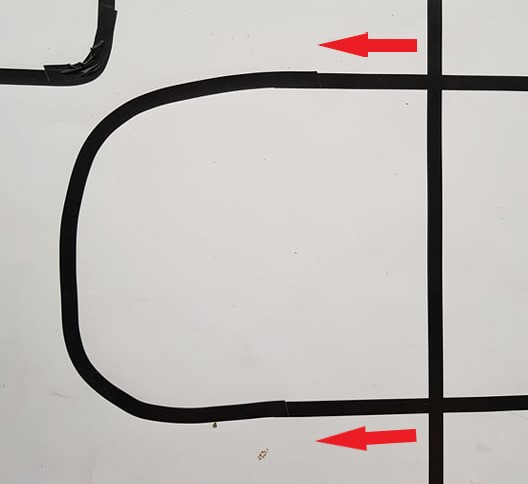
\includegraphics[width=0.9\textwidth]{figures/experiment_line_follower/line_follower_swing1.jpg}
        \caption{Swing 1}
        \label{fig:line_follower_swing1}
    \end{subfigure}%
    \begin{subfigure}{0.5\textwidth}
        \centering
        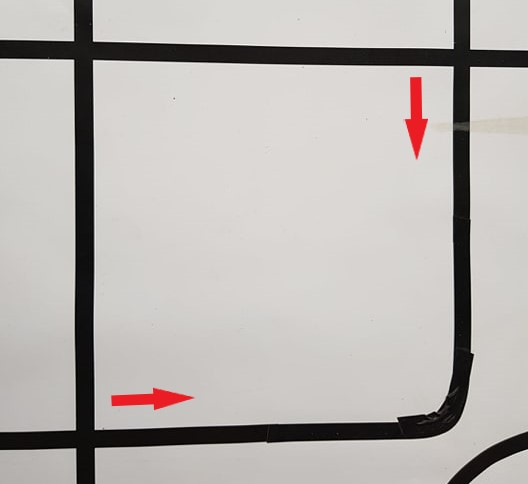
\includegraphics[width=0.9\textwidth]{figures/experiment_line_follower/line_follower_swing2.jpg}
        \caption{Swing 2}
        \label{fig:line_follower_swing2}
    \end{subfigure}
    \caption{Swings}
    \label{fig:line_follower}
\end{figure}
\subsection*{Results of the Experiment}
\todo{do the test}

\begin{table}[H]
\centering
\begin{tabular}{|c|c|c|c|c|}
\hline
 & \multicolumn{2}{c|}{Cloudy} & \multicolumn{2}{c|}{Sunny} \\ \hline
 & Passed & Failed & Passed & Failed \\ \hline
Swing 1 & $20$ & $0$ &  &  \\ \hline
Swing 2 & $20$ & $0$  &  &  \\ \hline
\end{tabular}
\caption{Results}
\label{tab:follow_line_results}
\end{table}

\section{Experiment: Detection of Intersection on the Map} \label{app:intersection}
The whereabouts of the robot on the map is essential to solve the puzzle. Therefore, a routine which uses the two color sensors to detect an intersection is created and tested. 

\subsection*{Results of the Experiment} \todo{do the test}

\section{Experiment: Turning in the Intersections} \label{app:turning}
To move around on the map the robot must be able to go left, right, backwards and forwards in an intersection. Thus, a routine that controls the two large motors is develop and tested. The results of the experiment are shown below.

\subsection*{Results of the Experiment}
\todo{do the test}

\end{document}